\documentclass[12pt]{article}

\usepackage[margin=1in]{geometry} % 1-inch margins
\usepackage{times}                % Times (Times New Roman–like) font
\usepackage{fancyhdr}             % Custom headers/footers
\usepackage{graphicx}             % For including images
\usepackage{titlesec}             % Section formatting
\usepackage{listings}             % For displaying code
\usepackage{xcolor}               % For custom colors
\usepackage{caption}
\usepackage{setspace}             % FOR 1.5 LINE SPACING

\pagestyle{fancy}
\fancyhf{}

% Header
\fancyhead[R]{Saksham AI: Multilingual Virtual Interviewer}

% Footer
\fancyfoot[L]{Pillai HOC College of Engineering \& Technology (Autonomous), Rasayani}
\fancyfoot[R]{\thepage}

% Header/Footer lines
\renewcommand{\headrulewidth}{0.4pt}
\renewcommand{\footrulewidth}{0.4pt}

% Paragraph Formatting
\setlength{\parindent}{1.5em}
\setlength{\parskip}{0em}

% 1.5 LINE SPACING
\onehalfspacing

% Code style
\lstdefinestyle{mystyle}{
    backgroundcolor=\color{white},   
    commentstyle=\color{gray},
    keywordstyle=\color{gray},
    numberstyle=\tiny\color{gray},
    stringstyle=\color{gray},
    basicstyle=\ttfamily\footnotesize,
    breaklines=true,
    captionpos=b,
    keepspaces=true,
    showspaces=false,
    showstringspaces=false,
    showtabs=false,
    tabsize=2
}

\lstset{style=mystyle}

\begin{document}

\setcounter{page}{33}

\vspace*{\fill}

\begin{center}
{\Large \bf Chapter 7}\\[2em]
{\Large \bf Implemented System}
\end{center}

\vspace*{\fill}

\newpage

\setcounter{section}{7}

\subsection{System Architecture}

\vspace{10pt}

\noindent The Fig. 7.1 illustrates how the frontend of the Multilingual AI Virtual Interviewer system routes user requests to the central processing system based on different interactions. When a candidate initiates an interview or an administrator accesses reports, the requests are forwarded to the core backend for processing. The backend invokes specialized components such as the Interview Module to manage the interview session flow and the Administration Module to handle reporting and access control. The business logic coordinates the overall workflow by utilizing the Language Processing Module to translate and analyze multilingual inputs and the AI Evaluation Module to assess the candidate’s responses. The Data Interface functions as the database management layer, performing CRUD (Create, Read, Update, Delete) operations across various storage systems, including the User Database, Question Repository, Evaluation Data, and Analytics Data. After processing, the backend retrieves the required information from the databases and sends responses back to the frontend, updating the user interface in real time to support the live interview experience for candidates or to display comprehensive evaluation dashboards for administrators.
\vspace{20pt}
\begin{figure}[htbp]
\centering
\renewcommand{\thefigure}{7.1}
\fbox{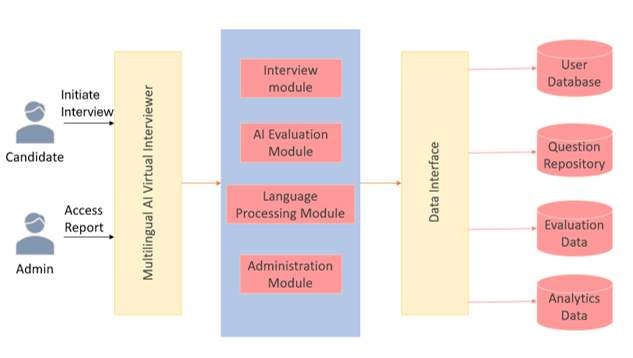
\includegraphics[width=1.0\textwidth]{SYSTEM ARCHI .png}}
\captionsetup{labelformat=empty}
\caption{Figure \thefigure: System Architecture}
\end{figure}

\newpage

\subsection{Sample code}

\vspace{10pt}

Below is the Python (Flask-based) backend code for the implemented Multilingual Virtual Interviewer system:

\begin{lstlisting}[language=Arduino]

from flask import Flask, render_template, request, jsonify, session, redirect, url_for
import os, secrets
from datetime import datetime
from config import Config
from models.ai_interviewer import AIInterviewer
from models.resume_analyzer import ResumeAnalyzer
from models.speech_processor import SpeechProcessor
from models.question_generator import QuestionGenerator
from utils.translator import MultilingualSupport
from utils.helpers import allowed_file

app = Flask(__name__)
app.config.from_object(Config)
os.makedirs(app.config.get('UPLOAD_FOLDER', 'uploads'), exist_ok=True)

# Initialize AI components
ai_interviewer = AIInterviewer()
resume_analyzer = ResumeAnalyzer()
speech_processor = SpeechProcessor()
question_generator = QuestionGenerator()
multilingual_support = MultilingualSupport()

@app.after_request
def after_request(response):
    response.headers.update({
        'Access-Control-Allow-Origin': '*',
        'Access-Control-Allow-Headers': 'Content-Type,Authorization',
        'Access-Control-Allow-Methods': 'GET,PUT,POST,DELETE,OPTIONS'
    })
    return response

# Automatically injects language variables into ALL templates
@app.context_processor
def inject_language_context():
    lang = session.get('language', 'en')
    return dict(
        current_lang=lang,
        translations=multilingual_support.get_ui_translations(lang),
        supported_languages=multilingual_support.SUPPORTED_LANGUAGES
    )

@app.route('/')
def index(): return render_template('index.html')

@app.route('/chatbot')
def chatbot_page(): return render_template('chatbot.html')

@app.route('/set_language/<lang>')
def set_language(lang):
    if lang in multilingual_support.SUPPORTED_LANGUAGES: session['language'] = lang
    return redirect(request.referrer or url_for('index'))

@app.route('/translate_text', methods=['POST'])
def translate_text():
    data = request.json
    return jsonify({'translated_text': multilingual_support.translate_text(
        data.get('text', ''), data.get('target_lang', 'en'), data.get('source_lang', 'auto')
    )})

@app.route('/analyze_resume', methods=['GET', 'POST'])
def analyze_resume():
    if request.method == 'POST':
        file = request.files.get('resume')
        if file and allowed_file(file.filename):
            try:
                filepath = os.path.join(app.config['UPLOAD_FOLDER'], f"{secrets.token_hex(8)}_{file.filename}")
                file.save(filepath)
                session['resume_analysis'] = resume_analyzer.analyze_resume_file(filepath)
                return render_template('resume_analysis.html', analysis=session['resume_analysis'])
            except Exception as e:
                return jsonify({'error': str(e)}), 500
        return jsonify({'error': 'Invalid file'}), 400
    return render_template('resume_analysis.html')

@app.route('/start_video_interview', methods=['POST'])
def start_video_interview():
    lang = session.get('language', 'en')
    job_role = request.form.get('job_role', 'software_engineer')
    resume_analysis = session.get('resume_analysis', {})
    
    questions = question_generator.generate_questions(job_role, resume_analysis)
    if lang != 'en': questions = multilingual_support.translate_questions(questions, lang)
    
    session.update({
        'interview_id': secrets.token_hex(16), 'current_question': 0, 'score': 0,
        'responses': [], 'questions': questions, 'job_role': job_role,
        'start_time': datetime.now().isoformat(), 'enable_voice': True, 'language': lang
    })
    return redirect(url_for('video_interview'))

@app.route('/video_interview')
def video_interview():
    if 'interview_id' not in session: return redirect(url_for('index'))
    return render_template('video_interview.html', enable_voice=session.get('enable_voice', True))

@app.route('/interview_room')
def interview_room():
    if 'interview_id' not in session: return redirect(url_for('index'))
    current_q, questions = session['current_question'], session['questions']
    
    if current_q >= len(questions): return redirect(url_for('results'))
    return render_template('interview_room.html', question=questions[current_q], 
                           question_num=current_q + 1, total_questions=len(questions), 
                           enable_voice=session.get('enable_voice', True))

@app.route('/submit_answer', methods=['POST'])
def submit_answer():
    if 'interview_id' not in session: return jsonify({'error': 'No active interview'}), 400
    
    current_q, questions = session['current_question'], session['questions']
    if current_q >= len(questions): return jsonify({'completed': True})

    score, feedback, analysis = ai_interviewer.analyze_answer(
        session['job_role'], current_q, request.form.get('answer', ''), session.get('resume_analysis', {})
    )
    
    # Generate dynamic feedback
    prefixes = {8: "Excellent!", 6: "Good job.", 4: "Okay.", 0: "I see."}
    prefix = next(p for s, p in prefixes.items() if score >= s)
    ai_feedback = f"{prefix} {feedback}"
    
    if session.get('language', 'en') != 'en':
        ai_feedback = multilingual_support.translate_feedback(ai_feedback, session['language'])

    session['responses'].append({
        'question': questions[current_q]['question'], 'answer': request.form.get('answer', ''),
        'score': score, 'feedback': ai_feedback, 'detailed_analysis': analysis
    })
    session['score'] += score
    session['current_question'] += 1
    
    return jsonify({'next_question': session['current_question'], 'score': score, 
                    'feedback': ai_feedback, 'completed': session['current_question'] >= len(questions)})

@app.route('/process_voice', methods=['POST'])
def process_voice():
    if 'interview_id' not in session or 'audio' not in request.files: return jsonify({'error': 'Invalid request'}), 400
    try:
        text = speech_processor.speech_to_text(request.files['audio'])
        return jsonify({'success': True, 'text': text}) if text else jsonify({'success': False, 'error': 'Audio unclear'})
    except Exception as e:
        return jsonify({'success': False, 'error': str(e)})

@app.route('/results')
def results():
    if 'interview_id' not in session: return redirect(url_for('index'))
    total_score, max_possible = session['score'], len(session['responses']) * 10
    
    feedback = ai_interviewer.generate_overall_feedback(session['responses'], session.get('resume_analysis', {}))
    if session.get('language', 'en') != 'en':
        feedback = multilingual_support.translate_feedback(feedback, session['language'])
        
    return render_template('results.html', score=total_score, 
                           percentage=(total_score / max_possible * 100) if max_possible else 0,
                           responses=session['responses'], overall_feedback=feedback)

if __name__ == '__main__':
    print("�� Running with HTTPS! Camera and microphone should work now.")
    print("�� Make sure to access via: https://localhost:5000")
    # 'adhoc' automatically generates a temporary SSL certificate!
    app.run(debug=True, ssl_context='adhoc', host='0.0.0.0', port=5000)


\end{lstlisting}

\end{document}